This section discusses the output layer of the work cell system and how each component is going to interact with  data inputs to perform the task of industrial painting. The primary goal of this layer is to receive signals from the processing layer and perform the necessary operations like moving the robotic arm/linear rail, execute the painting task, and illuminate the safety light tower.


\subsection{Robot}
This layer consists of the robot subsystem, which includes the Mitsubishi RV-8CRL robotic arm and the additional axis linear rail.

\begin{figure}[h!]
	\centering
 	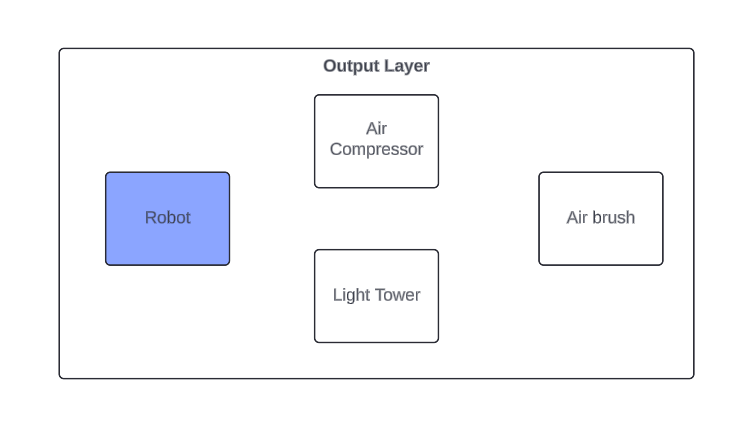
\includegraphics[width=0.60\textwidth]{images/Output_robot.png}
 \caption{Robot subsystem}
\end{figure}

\subsubsection{Assumptions}
The robotic arm provided by Mitsubishi is functional and abides to its specifications as provided by Mitsubishi documentation. We also assume the CR-800 controller is compatible with the robot and linear rail, and communication between the components is ensured through the RT Toolbox software stored on the host PC.

\subsubsection{Responsibilities}
The robot is responsible for movement and engaging in painting. Movement can be achieved through the robotic arm's 6 joints, as well as the additional 7th axis linear rail. The robot receives movement commands from the host PC and/or the robot controller's 'Operation Panel' (OP). The robot also houses the pneumatic line.
\subsubsection{Subsystem Interfaces}
\begin {table}[H]
\caption {Subsystem interfaces}
\begin{center}
    \begin{tabular}{ | p{1cm} | p{4cm} | p{5cm} | p{3cm} |}
    \hline
    ID & Description & Inputs & Outputs \\ \hline
    \#01 & Joint control & \pbox{5cm}{RT Toolbox program \\ Operation Panel} & \pbox{3cm}{Robot movement}  \\ \hline
    \#02 & Robot errors & \pbox{5cm}{Internal signals} & \pbox{3cm}{CR-800 controller}  \\ \hline
    \#03 & Pneumatic line & \pbox{5cm}{Base air hose} & \pbox{3cm}{Forearm airhose}  \\ \hline

    \end{tabular}
\end{center}
\end{table}

\subsection{Air Compressor}
An air compressor is a machine that takes ambient air from surroundings and discharges it at a higher pressure.

\begin{figure}[h!]
	\centering
 	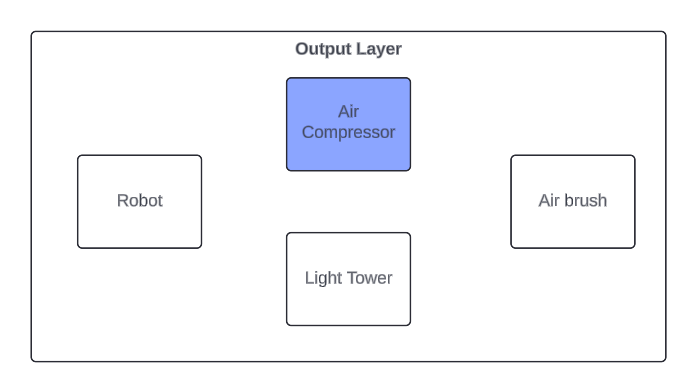
\includegraphics[width=0.60\textwidth]{images/Output_Compressor.png}
 \caption{Air Compressor subsytem}
\end{figure}

\subsubsection{Assumptions}
The primary role of an air compressor is to provide sufficient air pressure for spraying purposes.

\subsubsection{Responsibilities}
The electrical connection between the air compressor and the PLC ensures their communication. Additionally, the pneumatic lines run through the robot arm, maintaining the connection between the air brush and the air compressor.

\subsubsection{Subsystem Interfaces}
\begin {table}[H]
\caption {Subsystem interfaces}
\begin{center}
    \begin{tabular}{ | p{1cm} | p{6cm} | p{3cm} | p{4cm} |}
    \hline
    ID & Description & Inputs & Outputs \\ \hline
    \#04 & Sprays paint & \pbox{3cm}{PLC} & \pbox{4cm}{air pressure to air brush}
    \\\hline
    
    \end{tabular}
\end{center}
\end{table}


\subsection{Light Tower}
An industrial light tower system, typically used in a working cell or industrial setting, serves several essential responsibilities to ensure the efficient and safe operation of the workspace. The specific responsibilities of an industrial light tower system may vary depending on the application. For our system, it serves as an inference to the work environment as it indicates different modes with colored LEDs as get input from the controller and outputs as LEDs.

\begin{figure}[h!]
	\centering
 	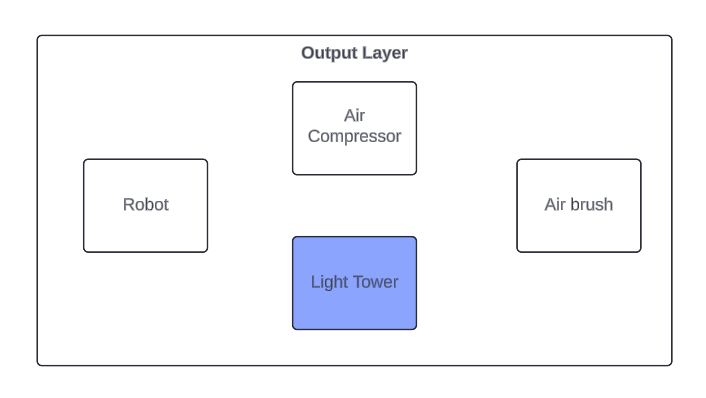
\includegraphics[width=0.60\textwidth]{images/Output_tower.png}
 \caption{Light tower subsystem}
\end{figure}

\subsubsection{Assumptions}
The "Light tower" subsystem assumes that it will receive status information from the PLC about the working status of the robot arm. It is assumed that this will be a reliable signal or interface to indicate the status of the working cell.

\subsubsection{Responsibilities}
Signaling and Alerts: Industrial light tower systems often include signal lights or beacons. These lights can be used to convey information or alerts to workers or nearby personnel. Common signals include indicating when a machine is running, signaling the need for maintenance or repair, or warning of specific hazards or emergencies.
Status Indication: The light tower system can provide status indications for machines or equipment within the working cell. 
Safety: Ensuring the safety of workers is a primary responsibility. Light towers can be programmed to flash or change colors to draw attention to potential safety hazards, such as moving equipment or areas that require caution.

\subsubsection{Subsystem Interfaces}
\begin {table}[H]
\caption {Subsystem interfaces} 
\begin{center}
    \begin{tabular}{ | p{1cm} | p{6cm} | p{3cm} | p{3cm} |}
    \hline
    ID & Description & Inputs & Outputs \\ \hline
    \#05 & Stop Operation & \pbox{3cm}{E stops} & \pbox{3cm}{red led signal}  \\ \hline
    \#06 & Calibrating & \pbox{3cm}{PLC} & \pbox{3cm}{yellow led signal}  \\ \hline
    \#07 & Regular operation & \pbox{3cm}{PLC} & \pbox{3cm}{green led signal}  \\ \hline
    \end{tabular}
\end{center}
\end{table}

\subsection{Air brush}
An airbrush is a versatile tool used by artists, creators, and hobbyists to apply color to various surfaces

\begin{figure}[h!]
	\centering
 	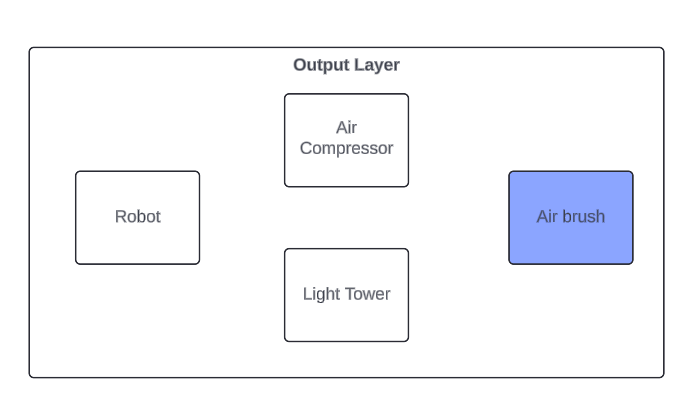
\includegraphics[width=0.60\textwidth]{images/Output_brush.png}
 \caption{Air brush subsystem}
\end{figure}

\subsubsection{Assumptions}
Air brush expects air pressure from air compressor as per the pattern requirement.

\subsubsection{Responsibilities}
The airbrush's role is to apply paint while the robot moves in a predetermined pattern as per its programming.

\subsubsection{Subsystem Interfaces}
\begin {table}[H]
\caption {Subsystem interfaces} 
\begin{center}
    \begin{tabular}{ | p{1cm} | p{6cm} | p{3cm} | p{3cm} |}
    \hline
    ID & Description & Inputs & Outputs \\ \hline
    \#08 & Tool for spraying & \pbox{3cm}{Air compressor} & \pbox{3cm}{sprays paint}  \\ \hline
    \end{tabular}
\end{center}
\end{table}